%%%%%%%%%%%%%%%%%%%%%%%%%%%%%%%%%%%%%%%%%
% Beamer Presentation
% LaTeX Template
% Version 1.0 (10/11/12)
%
% This template has been downloaded from:
% http://www.LaTeXTemplates.com
%
% License:
% CC BY-NC-SA 3.0 (http://creativecommons.org/licenses/by-nc-sa/3.0/)
%
%%%%%%%%%%%%%%%%%%%%%%%%%%%%%%%%%%%%%%%%%

%----------------------------------------------------------------------------------------
%	PACKAGES AND THEMES
%----------------------------------------------------------------------------------------

\documentclass{beamer}

\mode<presentation> {

\usetheme{Madrid}

\setbeamertemplate{navigation symbols}{} % To remove the navigation symbols from the bottom of all slides uncomment this line
}

\usepackage{graphicx} % Allows including images
\usepackage{booktabs} % Allows the use of \toprule, \midrule and \bottomrule in tables
\usepackage{amsmath}
\usepackage{amsfonts}
\usepackage{amssymb}
\usepackage{url}
\usepackage{color}
\usepackage{calc}
\usepackage[T1]{fontenc}
\usepackage[french]{babel}
\usepackage[utf8]{inputenc}
\usepackage{pifont}
\usepackage{fancyvrb}
\usepackage{xparse}
\usepackage{tgcursor}

\newlength{\charwidth}
\setlength{\charwidth}{\widthof{\S}}
\newcommand{\uline}{\underline{\hspace{2\charwidth}}}
\newcommand{\Sn}{\mathrm{Sn}}


\newenvironment{repl}
 {\VerbatimEnvironment
  \let\FancyVerbFormatLine\shellformatline
  \Verbatim}
 {\endVerbatim}

\ExplSyntaxOn
\NewDocumentCommand{\shellformatline}{m}
 {
  \str_if_eq_x:nnTF { \tl_head:n { #1 } } { > }
   { sage: \bfseries \tl_tail:n { #1 } }
   { #1 }
 }
\ExplSyntaxOff
%----------------------------------------------------------------------------------------
%	TITLE PAGE
%----------------------------------------------------------------------------------------

\title[Suites P-récursives]{Projet SFPN : Manipulation de suites P-récursives avec SageMath}

\author[M. Caristan \& A. Lamoureux]{Mathis \textsc{Caristan} \& Aurélien \textsc{Lamoureux}\\
{\scriptsize Sous la responsabilité de Marc \textsc{Mezzarobba}}}
\institute[UPMC]{Université Pierre \& Marie Curie}
\date{29/05/2017}

\begin{document}

\begin{frame}
\titlepage % Print the title page as the first slide
\end{frame}

\begin{frame}
%\frametitle{} % Table of contents slide, comment this block out to remove it
\tableofcontents % Throughout your presentation, if you choose to use \section{} and \subsection{} commands, these will automatically be printed on this slide as an overview of your presentation
\end{frame}

%----------------------------------------------------------------------------------------
%	PRESENTATION SLIDES
%----------------------------------------------------------------------------------------
%%%%%%%%%%%%%%%%%%%%%%%%%
\section{Introduction}%%%
%%%%%%%%%%%%%%%%%%%%%%%%%

\begin{frame}
\frametitle{Quelques objets mathématiques}
\begin{minipage}{0.45\textwidth} \begin{center}
    \begin{figure}\begin{center}
        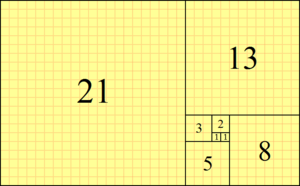
\includegraphics[scale=0.5]{fibo}
    \end{center} \end{figure}
    $F_{n+2} - F_{n+1} - F_n = 0$
\end{center} \end{minipage}
\hspace{2ex}
\begin{minipage}{0.45\textwidth} \begin{center}
    \begin{figure}\begin{center}
        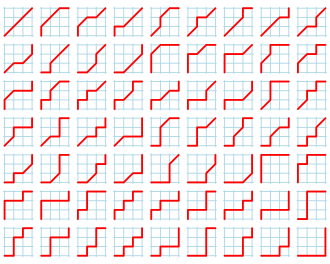
\includegraphics[scale=0.5]{delannoy}
    \end{center} \end{figure}
    $D(m,n) = D(m-1,n) + D(m-1,n-1) + D(m,n-1)$
\end{center} \end{minipage}
\vspace{1cm} \pause
\begin{center}
{\large mais aussi la fonction factorielle, le binôme de Newton, le nombre de partitions d'un
    nombre...}
\end{center}
\end{frame}

\begin{frame}
\frametitle{Contexte \& problématique}
\begin{center}
Les suites P-récursives sont des objets couramment utilisés en mathématiques et en sciences.
\begin{alertblock}{Problématique}
    \begin{itemize}
        \item \textbf{\large La question se pose de comment représenter et manipuler
                informatiquement ces objets.}
        \item Les suites sont infinies.
    \end{itemize}
\end{alertblock}
\pause
\begin{exampleblock}{Solution}
    Il est nécessaire d'utiliser les propriétés mathématiques des suites P-récursives.
\end{exampleblock}
\end{center}
\end{frame}
        
%------------------------------------------------

\begin{frame}
\frametitle{Suites P-récursives}
\begin{center}
    \vspace{-2ex}
\begin{block}{Définition formelle} \begin{center}
    Une suite P-récursive sur un corps $\mathbb K$ vérifie la propriété suivante :
    \begin{equation*}
        \sum^k_{i=0} P_i(n)u_{n+i} = 0
    \end{equation*}
    où les $P_i$ sont des polynômes en $n$, et $k$ est l'ordre de la récurrence.
\end{center} \end{block}
Une suite P-récursive peut être représentée exactement avec sa relation de récurrence,
et ses conditions initiales$^*$
\begin{exampleblock}{Exemples}
    \vspace{-2ex}
    \begin{eqnarray*}
        \text{Fibonacci : } F_{n+2} - F_{n+1} - F_n = 0,  \qquad &F_0 = 0, F_1 = 1 \\
        \text{Factorielle : } (n+1)! - (n+1)(n!) = 0,  \qquad &0! = 1 \\
        \textit{Fonction anodine : } (n-2)u_{n+1} - u_n = 0,  \qquad &u_0 = 2\\
    \end{eqnarray*}
    \vspace{-7ex}
\end{exampleblock}
\end{center}
\end{frame}

%------------------------------------------------

\begin{frame}
\frametitle{SageMath \& Python}
\begin{center}
\begin{block}{SageMath, qu'est-ce que c'est?}
    \begin{itemize}
        \item Un logiciel de calcul formel
        \item Open source
        \item Construit sur un ensmble d'outil pré-éxistant et Python
        \item Basé sur Python
        \item Doté d'une syntaxe spécifique pour la ligne de commande
    \end{itemize}
\end{block}
\begin{block}{Python?}
    \begin{itemize}
        \item {\large C'est le langage sur lequel est basé Sage}
        \item Python 2.7.9
        \item Les idiomes Sage sont transformés en Python pur
        \item Possibilité d'écrire des modules pour Sage en Python
    \end{itemize}
\end{block}
\end{center}
\end{frame}

%------------------------------------------------

\begin{frame}
\frametitle{Les algèbres d'Ore}
\begin{center}
\begin{block}{Algèbres d'Ore}
    \begin{itemize}
        \item Bien plus vaste que le cadre de ce projet
        \item Déterminée par un anneau, et un opérateur
    \end{itemize}
\end{block}
\begin{exampleblock}{Exemples}
    \begin{itemize}
        \item L'anneau sera $\mathbb R[x]$
        \item $\text{L'opérateur de décalage } \Sn \colon n \mapsto n+1$
        \item On associe un opérateur d'annihilation à une suite :
            \vspace{-2ex}
            \begin{eqnarray*}
                \text{Fibonacci : } &(\Sn^2 - \Sn - 1)F_n = 0\\
                \text{Factorielle : } &(\Sn - (n+1))(n!) = 0\\
                (u_n)_{n\in\mathbb N}~\colon &((n-2)\Sn - 1)u_n = 0
            \end{eqnarray*}
        \item Les annihilateurs sont des polynômes en $n$ et $\Sn$.
        \item On utilise la bibliothèque \textsc{OreAlgebra} comme boîte à outils.
    \end{itemize}
\end{exampleblock}
\end{center}
\end{frame}

%------------------------------------------------
%%%%%%%%%%%%%%%%%%%%%%%%%%%%%%
\section{Contenu du module}%%%
%%%%%%%%%%%%%%%%%%%%%%%%%%%%%%

\begin{frame}
\frametitle{Présentation du module}
\begin{center}
\begin{alertblock}{Problématique}
    Créer un module facilitant la manipulation des suites p-récursives.
\end{alertblock}
\vspace{0.6cm}
\begin{block}{Caractéristiques}
    \begin{itemize}
        \item {\footnotesize En Python}
        \item Basé sur le modèle de programmation objet : une classe
        \item Surcharge d'opérateurs
        \item Des tests
    \end{itemize}
\end{block}
\vspace{0.6cm}
Notre classe n'étend aucune classe pré-éxistante.
\end{center}
\end{frame}


\begin{frame}
\frametitle{Objectifs du module}
\begin{center}
\begin{block}{Objectifs principaux}
    \begin{itemize}
        \item Un constructeur
        \item Les opérations $+$ et $\times$
        \item Une fonction pour calculer un élément
    \end{itemize}
\end{block}
\pause
\begin{minipage}{0.45\textwidth} \begin{center}
    \begin{block}{Objectifs importants}
        \begin{itemize}
            \item Travailler dans différents anneaux
            \item Des suites constantes
            \item Une méthode qui teste si une suite est constante
            \item Les tests d'égalité/inégalité
            \item Un constructeur qui devine la récurrence
        \end{itemize}
    \end{block}
\end{center} \end{minipage}
\hspace{2ex} \pause
\begin{minipage}{0.45\textwidth} \begin{center}
    \begin{block}{Objectifs secondaires}
        \begin{itemize}
            \item Les opérateurs $<<$ et $>>$
            \item Un itérateur (infini)
            \item La division par une constante
            \item Un constructeur à partir d'une expression symbolique
        \end{itemize}
    \end{block}
\end{center} \end{minipage}
\end{center}
\end{frame}

%------------------------------------------------

\begin{frame}[fragile]
\frametitle{Constructeur}
\begin{center}
\begin{exampleblock}{Comportement par défaut}
    \begin{repl}
> fibo = PRecSequence ({0:0,1:1}, Sn**2 - Sn - 1)
> fact = PRecSequence ({0:1}, Sn - n - 1)
> u = PRecSequence ({0:2}, (n-2)*Sn - 1)
    \end{repl}
\end{exampleblock}
\begin{block}{Comportements secondaires}
    D'autres comportements sont possibles, grâce aux arguments optionnels de Python
    \begin{itemize}
        \item Création d'une suite constante :
            \begin{repl}
> u_const = PRecSequence (const=5)
            \end{repl}
        \item "Guessing" a partir d'une liste d'éléments:
            \begin{repl}
> fib_guess = PRecSequence ([0,1,1,2,3,5,8],R)
> print fib_guess.annihilator
-Sn^2 + Sn + 1
            \end{repl}
    \end{itemize}
\end{block}
\end{center}
\end{frame}

%------------------------------------------------

\begin{frame}
\frametitle{Constructeur - Problèmes}
\begin{center}
\begin{alertblock}{Les valeurs singulières}
    Lorsque le polynôme dominant a des racines dans $\mathbb Z$ :
    \begin{align*}
        (n-2)u_{n+1} - u_n = 0 &\qquad u_0=2\\
        -2*u_1 - u_0 = 0 &\qquad\Rightarrow u_1 = -1\\
        -u_2 - u_1 = 0 &\qquad\Rightarrow u_2 = 1\\
        0*u_3 - u_2 = 0 &\qquad\Rightarrow u_2 = 0, u_3 =???\\
    \end{align*}
\end{alertblock}
\pause
\begin{exampleblock}{Les conditions initiales supplémentaires}
    Il est nécessaire de permettre de fixer des conditions supplémentaires.\\
    \pause
    \textbf{1\iere{} idée} : Obliger l'utilisateur à renseigner les valeurs dégénérées. Obliger 
    l'utilisateur à saisir \textit{toutes} les valeurs jusqu'à la dernière racine.\\
    \pause
    \textbf{2\ieme{} idée} : Lever des exceptions
\end{exampleblock}
\end{center}
\end{frame}

%------------------------------------------------

\begin{frame}[fragile]
\frametitle{Constructeur - Conditions initiales}
\begin{center}
{\large Comment traiter les conditions initiales supplémentaires?}
\begin{block}{Les valeurs n'influent pas le calcul}
    \begin{repl}
> PRecSequence ({0:0,1:1,5:6}, Sn**2 - Sn - 1)
    \end{repl}
    Les valeurs de la suite sont $(0,1,1,2,3,6,8,13,21\ldots)$
\end{block}
\begin{block}{Les valeurs influent sur les termes suivants}
    \begin{repl}
> PRecSequence ({0:0,1:1,5:6}, Sn**2 - Sn - 1)
    \end{repl}
    Les valeurs de la suite sont $(0,1,1,2,3,6,9,15,24\ldots)$
\end{block}
\end{center}
\end{frame}

%------------------------------------------------

\begin{frame}
\frametitle{Accéder à un élément de la suite}
\begin{center}
Il faut surcharger l'opérateur \texttt{\uline getitem\uline}, qui permet en Python
d'accéder à l'élément $n$ : \texttt{fibo[$n$]} ou \texttt{fibo[$n_1:n_2$]}.
\begin{block}{Première méthode : \texttt{to\_list}}
    La classe de notre annihilateur propose \texttt{to\_list}, qui calcule récursivement tous
    les termes jusqu'à $n$.
    \begin{itemize}
        \item Facile à implémenter
        \item Mais lent
    \end{itemize}
\end{block}
\begin{block}{Deuxième méthode : \texttt{forward\_matrix\_bsplit}}
    Utiliser l'algèbre linéaire pour calculer directement le terme $n$
    \begin{itemize}
        \item Théoriquement plus rapide
        \item Souffre d'un temps d'amorce
    \end{itemize}
\end{block}
\end{center}
\end{frame}

%------------------------------------------------

\begin{frame}
\frametitle{Optimiser \texttt{\uline getitem \uline}}
\begin{center}
Nous avons comparé les temps d'exécution pour les deux méthodes.
\begin{figure}
    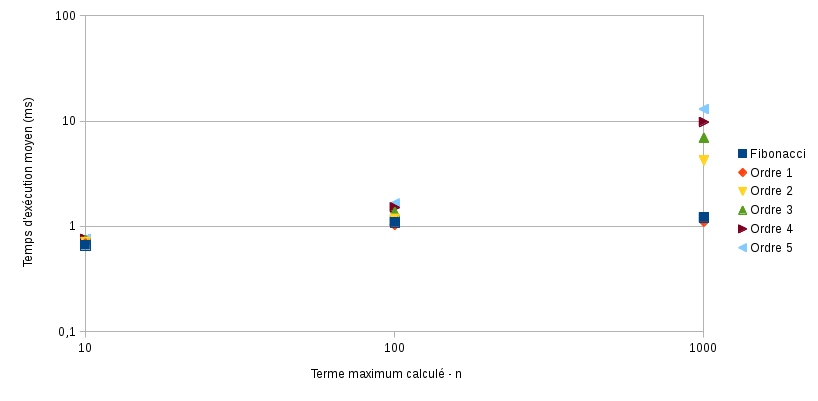
\includegraphics[scale=0.4]{graphe}
\end{figure}
{\scriptsize Rapport du temps avec \texttt{to\_list} sur le temps avec 
\texttt{forward\_matrix\_bsplit}.}\\
\vspace{1cm}
La seconde méthode est déjà plus efficace pour des valeurs de l'ordre de 100.
\end{center}
\end{frame}

%------------------------------------------------

\begin{frame}
\frametitle{Addition et multiplication}
\begin{center}
\begin{block}{Principe}
    \begin{itemize}
        \item Trouver un operateur qui annule les deux termes
        \item Trouver de nouvelle conditions initials
    \end{itemize}
\end{block}
\pause
\begin{alertblock}{Problèmes}
    \begin{itemize}
        \item Comment trouver cet opérateur ?
        \item Comment faire si cet opérateur a des racine sur son coefficient dominant?
    \end{itemize}
\end{alertblock}
\end{center}
\end{frame}

%------------------------------------------------

%------------------------------------------------

%%%   \begin{frame}
%%%   \frametitle{Addition et multiplication}
%%%   \begin{center}
%%%   \begin{exampleblock}{Utiliser les facteurs}
%%%       \begin{align*}
%%%           \textnormal{Const : } &C_{n+1} - C_n = 0,\qquad E_0 = 2,\\
%%%           \textnormal{Fibonacci : } &F_{n+2} - F_{n+1} - F_n = 0,\qquad F_0=0, F_1=1\\
%%%           \textnormal{Leur Sommme : } &S_{n+3} - 2*S_{n+2} + S_n = 0 \\
%%%           &S_0 = 2, S_1 = 3, S_2 = 3\\
%%%       \end{align*}\\
%%%       $Const.lclm(Fibonacci)= Sn^3 - 2*Sn^2 + 1  $\\
%%%       l'opérateur annule les deux suites\\
%%%       [0, 1, 1, 2, 3, 5, 8, 13, 21, 34,...]\\
%%%       [2, 2, 2, 2, 2, 2, 2, 2, 2, 2,..]\\
%%%   \end{exampleblock}
%%%   \end{center}
%%%   \end{frame}
%%%   
%%%   %------------------------------------------------
%%%   \begin{frame}
%%%   \frametitle{Addition et multiplication - Procurer des conditions supplémentaires}
%%%   \begin{center}
%%%   \begin{alertblock}{Termes dégénérés dans les sommes/produits}
%%%       Le coefficient dominant de certains produits ou sommes ont des racines dans $\mathbb Z$.
%%%   \end{alertblock}
%%%   \begin{exampleblock}{Utiliser les facteurs}
%%%       \begin{align*}
%%%           \textnormal{Ent. Consec. : } &nE_{n+1} - (n+1)E_n = 0,\qquad E_0 = 0, N_1 = 1\\
%%%           \textnormal{Fibonacci : } &F_{n+2} - F_{n+1} - F_n = 0,\qquad F_0=0, F_1=1\\
%%%           \textnormal{Leur Sommme : } &(n - 1)D_{n+3} + (-2n + 1)D_{n+2} + D_{n+1} + nD_n = 0, \\
%%%           &D_0 = 0, D_1 = 2, D_2 = 3\\
%%%       \end{align*}\\
%%%       \vspace{-0.7cm}
%%%       $D_4$ est dégénéré, mais $E_4$ et $F_4$ existent.
%%%   \end{exampleblock}
%%%   \end{center}
%%%   \end{frame}

%------------------------------------------------

\begin{frame}
\frametitle{Autres fonctions}
\begin{center}
\emph{TODO}
\end{center}
\end{frame}





%%%   \begin{frame}
%%%   \frametitle{Bullet Points}
%%%   \begin{itemize}
%%%   \item Lorem ipsum dolor sit amet, consectetur adipiscing elit
%%%   \item Aliquam blandit faucibus nisi, sit amet dapibus enim tempus eu
%%%   \item Nulla commodo, erat quis gravida posuere, elit lacus lobortis est, quis porttitor odio mauris at libero
%%%   \item Nam cursus est eget velit posuere pellentesque
%%%   \item Vestibulum faucibus velit a augue condimentum quis convallis nulla gravida
%%%   \end{itemize}
%%%   \end{frame}
%%%   
%%%   %------------------------------------------------
%%%   
%%%   \begin{frame}
%%%   \frametitle{Blocks of Highlighted Text}
%%%   \begin{block}{Block 1}
%%%   Lorem ipsum dolor sit amet, consectetur adipiscing elit. Integer lectus nisl, ultricies in feugiat rutrum, porttitor sit amet augue. Aliquam ut tortor mauris. Sed volutpat ante purus, quis accumsan dolor.
%%%   \end{block}
%%%   
%%%   \begin{block}{Block 2}
%%%   Pellentesque sed tellus purus. Class aptent taciti sociosqu ad litora torquent per conubia nostra, per inceptos himenaeos. Vestibulum quis magna at risus dictum tempor eu vitae velit.
%%%   \end{block}
%%%   
%%%   \begin{block}{Block 3}
%%%   Suspendisse tincidunt sagittis gravida. Curabitur condimentum, enim sed venenatis rutrum, ipsum neque consectetur orci, sed blandit justo nisi ac lacus.
%%%   \end{block}
%%%   \end{frame}
%%%   
%%%   %------------------------------------------------
%%%   
%%%   \begin{frame}
%%%   \frametitle{Multiple Columns}
%%%   \begin{columns}[c] % The "c" option specifies centered vertical alignment while the "t" option is used for top vertical alignment
%%%   
%%%   \column{.45\textwidth} % Left column and width
%%%   \textbf{Heading}
%%%   \begin{enumerate}
%%%   \item Statement
%%%   \item Explanation
%%%   \item Example
%%%   \end{enumerate}
%%%   
%%%   \column{.5\textwidth} % Right column and width
%%%   Lorem ipsum dolor sit amet, consectetur adipiscing elit. Integer lectus nisl, ultricies in feugiat rutrum, porttitor sit amet augue. Aliquam ut tortor mauris. Sed volutpat ante purus, quis accumsan dolor.
%%%   
%%%   \end{columns}
%%%   \end{frame}
%%%   
%%%   %------------------------------------------------
%%%   
%%%   \begin{frame}
%%%   \frametitle{Table}
%%%   \begin{table}
%%%   \begin{tabular}{l l l}
%%%   \toprule
%%%   \textbf{Treatments} & \textbf{Response 1} & \textbf{Response 2}\\
%%%   \midrule
%%%   Treatment 1 & 0.0003262 & 0.562 \\
%%%   Treatment 2 & 0.0015681 & 0.910 \\
%%%   Treatment 3 & 0.0009271 & 0.296 \\
%%%   \bottomrule
%%%   \end{tabular}
%%%   \caption{Table caption}
%%%   \end{table}
%%%   \end{frame}
%%%   
%%%   %------------------------------------------------
%%%   
%%%   \begin{frame}
%%%   \frametitle{Theorem}
%%%   \begin{theorem}[Mass--energy equivalence]
%%%   $E = mc^2$
%%%   \end{theorem}
%%%   \end{frame}
%%%   
%%%   %------------------------------------------------
%%%   
%%%   \begin{frame}[fragile] % Need to use the fragile option when verbatim is used in the slide
%%%   \frametitle{Verbatim}
%%%   \begin{example}[Theorem Slide Code]
%%%   \begin{verbatim}
%%%   \begin{frame}
%%%   \frametitle{Theorem}
%%%   \begin{theorem}[Mass--energy equivalence]
%%%   $E = mc^2$
%%%   \end{theorem}
%%%   \end{frame}\end{verbatim}
%%%   \end{example}
%%%   \end{frame}
%%%   
%%%   %------------------------------------------------
%%%   
%%%   \begin{frame}
%%%   \frametitle{Figure}
%%%   Uncomment the code on this slide to include your own image from the same directory as the template .TeX file.
%%%   %\begin{figure}
%%%   %\includegraphics[width=0.8\linewidth]{test}
%%%   %\end{figure}
%%%   \end{frame}
%%%   
%%%   %------------------------------------------------
%%%   
%%%   \begin{frame}[fragile] % Need to use the fragile option when verbatim is used in the slide
%%%   \frametitle{Citation}
%%%   An example of the \verb|\cite| command to cite within the presentation:\\~
%%%   
%%%   This statement requires citation \cite{p1}.
%%%   \end{frame}
%%%   
%%%   %------------------------------------------------
%%%   
%%%   \begin{frame}
%%%   \frametitle{References}
%%%   \footnotesize{
%%%   \begin{thebibliography}{99} % Beamer does not support BibTeX so references must be inserted manually as below
%%%   \bibitem[Smith, 2012]{p1} John Smith (2012)
%%%   \newblock Title of the publication
%%%   \newblock \emph{Journal Name} 12(3), 45 -- 678.
%%%   \end{thebibliography}
%%%   }
%%%   \end{frame}
%%%   
%%%   %------------------------------------------------
%%%   
%%%   \begin{frame}
%%%   \Huge{\centerline{The End}}
%%%   \end{frame}

%----------------------------------------------------------------------------------------

\end{document} 
